
% ----------------------------------------------------------------------
\section{Results}
\label{sec:results}
% ----------------------------------------------------------------------

Using climate forcing from WorldClim data, the NCEP/NCAR, ERA-Iterim, CFSR and NARR reanalyses described in section~\ref{sec:climate} and the ice sheet model described in section~\ref{sec:model}, we run simulations of glacial inception and growth of the Cordilleran ice sheet using different temperature offsets.

\begin{figure*}[t]
	\vspace*{2mm}
	\begin{center}
		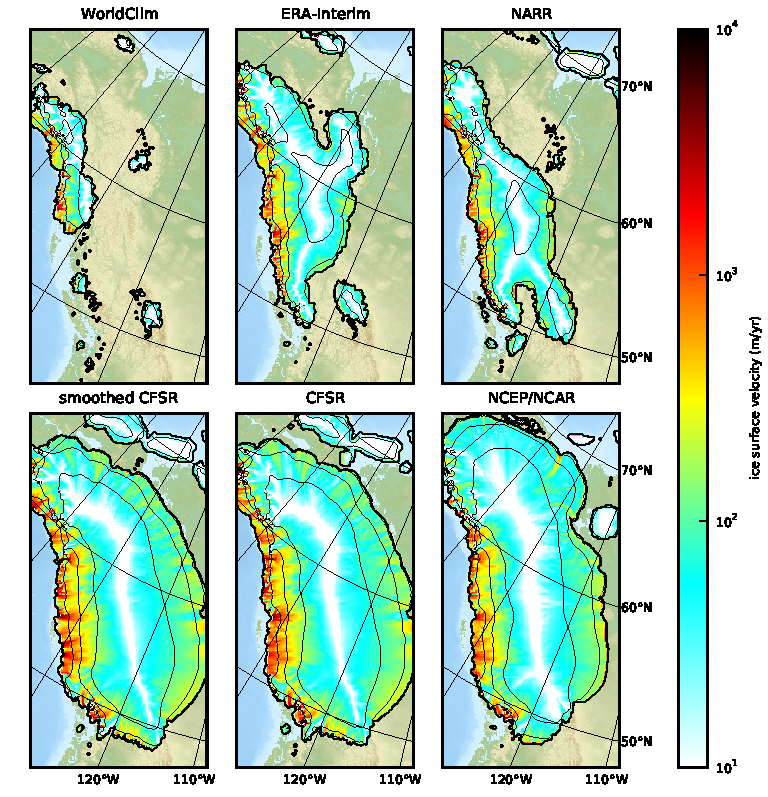
\includegraphics[width=13cm]{cordillera-climate-cool06}
	\end{center}
	\caption{Ice surface topography (black contours every 1000\,m) and velocity (\unit{m\,yr^{-1}}) after 10\,kyr under a climate 6\degC colder than present for each climate forcing.}
	\label{fig:cool06}
\end{figure*}

Figure~\ref{fig:cool06} shows the outcome of simulations run with a 6\degC temperature offset for each of the 6 climate forcings. In all simulations, ice accumulates and glaciers form as a result of the artificially cooled climate. Yet the magnitude of glaciation appears very different from one climate forcing to another. Whereas the NCAR and CFSR forcings produce a large ice sheet that covers most of the model domain land, the WorldClim, ERA-Interim and NARR forcings lead to more restrictive ice cover, bounded to mountain ice caps in the case of WorldClim data. The smoothing of CFSR precipitation data has limited visual effect on the resulting ice sheet geometry.

\begin{figure*}[t]
	\vspace*{2mm}
	\begin{center}
		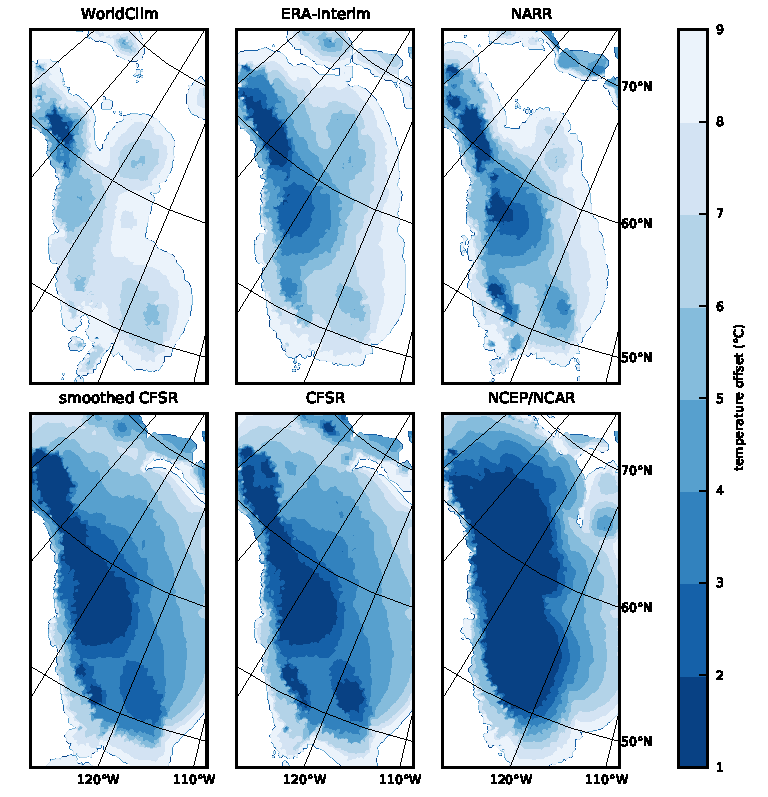
\includegraphics[width=13cm]{cordillera-climate-extent}
	\end{center}
	\caption{Extent of ice cover after 10\,kyr as a function of applied temperature offsets for each climate forcing.}
	\label{fig:extent}
\end{figure*}

As we aim to model an ice sheet approaching LGM size, and consider temperature offset as an unknown parameter in this study, we ran simulations using offset values ranging from 2 to 9\degC for each climate forcing.

Figure~\ref{fig:extent} shows the extent of ice cover at the end of each of these~(48) simulations, grouped by climate forcing. It is again visible that different forcings generally lead to very different final ice cover. Notably, for the smallest temperature offset value of 2\degC that was used, NCAR and CFSR simulations lead to an ice-sheet, whereas WorldClim, NARR and ERA-Interim produced local ice caps only, restricted to the Wrangell-St.~Elias mountains in the case of WorldClim, an area presently glaciated. Several of the NCAR and CFSR simulations produced oversized ice-sheets whose extent is primirily bounded by the model domain boundary conditions rather than physical processes. Differences in regional patterns can also be noted. For instance ERA-Interim ice sheets generally appear more northernly-centered than NARR ice sheets.

\begin{figure}[t]
	\vspace*{2mm}
	\begin{center}
		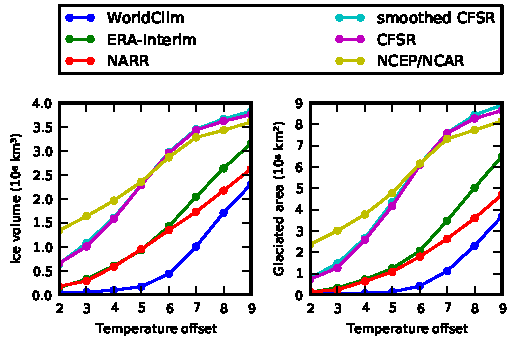
\includegraphics[width=9cm]{cordillera-climate-ivolarea}
	\end{center}
	\julien[inline]{I will make the figure readable in black-and-white and highlight markers corresponding to the ``best'' runs.}
	\caption{Total ice volume and glaciated area after 10\,kyr as a function of temperature offset and climate forcing.}
	\label{fig:ivolarea}
\end{figure}

Final ice volume and final ice coverage at the end of all simulations is quantified in Figure~\ref{fig:ivolarea}. The NCEP/NCAR and CFSR forcing lead to a much larger and more extensive glaciation than the ERA-Interim, NARR and WorldClim forcings. The ERA-Interim and NARR lead to similar ice volumes and glaciated areas, yet regional patterns are different, as shown by Figure~\ref{fig:extent}.

\begin{figure*}[t]
	\vspace*{2mm}
	\begin{center}
		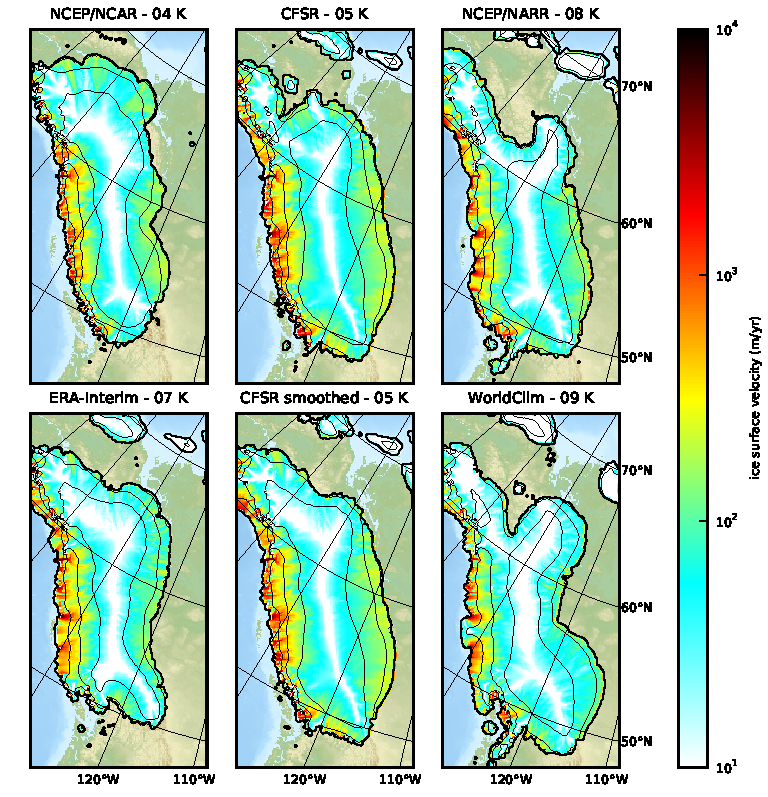
\includegraphics[width=13cm]{cordillera-climate-best}
	\end{center}
	\julien[inline]{I will to overlay the geomorphologic LGM ice margin so that it becomes easier to see which runs match it better.}
	\caption{Ice surface topography (black contours every 1000\,m) and velocity (\unit{m\,yr^{-1}}) after 10\,kyr using temperature offsets that lead to similar areas of ice cover for each climate forcing.}
	\label{fig:best}
\end{figure*}

To compare modelled ice sheets of similar size, we selected for each climate forcing the simulation that lead to a glaciated area closest to an arbitrary target of $4\,\times10^6\,\unit{km^2}$. These qualitative ``best'' runs are presented in Figure~\ref{fig:best} along the associated temperature offset values. We observe that although similar in size, the selected ice sheets are different in shape and flow patterns. More specifically, NCEP/NCAR, CFSR and ERA-Interim ice sheets cover large territories in Yukon and Alaska that where shown to have remained ice-free for at least several glacial cycles\citep{dukrodkin-1999,kaufman-manley-2004}.

